
\subsection{Single Lepton Top MC Modelling Validation from CR2}
\label{sec:cr2}


The \mt\ tail for single-lepton top events (\ttsl\ and single top) is dominated by jet resolution effects. The \W\ cannot be far off-shell because $\mW < \mtop$.
The modeling of the \mt\ tail from jet resolution effects can be studied
using \zjets\ data and MC samples.   However, as we will show below,
this test is statistically limited and can only be performed for the 
\met\ requirements corresponding to SRA and SRB.

\Z\ events are selected by requiring exactly 2 good leptons (satisfying ID
and isolation requirements) and requiring the \mll\ to be in the range
$81-101$ GeV. 
Events with additional isolated tracks are vetoed, as in Section~\ref{sec:tkveto}.
To reduce \ttbar\ backgrounds, events with a CSVM tag %H
are removed.
The positive lepton is treated as a neutrino and so is added to the MET: \met\ $\rightarrow$ \pt(\Lepp) + \met, 
and the \mt\ is recalculated with the negative lepton: \mt(\Lepm, \met).
The resulting ``pseudo-\mt'' is dominated by jet resolution effects, since no off-shell 
\Z\ production enters the sample due to the \mll\ requirement.
This section describes how well the MC predicts the tail of ``pseudo-\mt''. 

The underlying distributions are shown in Fig.~\ref{fig:cr2met}.
%and~\ref{fig:cr2mtrest}.   
We then perform the exact same type of Data/MC comparison and analysis as 
described for CR1 in Section~\ref{sec:cr1}.  For CR1 we collected
the data/MC tail information in 
Table~\ref{tab:cr1yields}; the equivalent for CR2 is
Table~\ref{tab:cr2yields} (for CR2 the statistics are not sufficient to split electrons and muons).
The last line of Table~\ref{tab:cr2yields} gives the data/MC scale factors
for the \ttbar\ lepton $+$ jets $M_T$ tail ($SFR_{top}$).  This is
calculated in the same way as $SFR_{wjets}$ of Table~\ref{tab:cr1yields}.
 Just as in CR1, there is an excess of data in the tails, as reflected
 in the values of $SFR_{top}$. There are insufficient events to derive scale factors for
$\met\ > 150$~GeV. As a result, the scale factors derived from CR2 are
not used for the central prediction of the single-lepton top
background. They serve as a valuable cross check of the predictions
described in Section~\ref{sec:ttp}. The single lepton top predictions
obtained for SRA and SRB using the $SFR_{top}$ values described here
are consistent with the default predictions.


\begin{table}[!h]
\begin{center}
{\footnotesize
\begin{tabular}{l||c|c||c|c}
\hline
Sample              & CR2PRESEL0 &CR2PRESEL1 & CR2A & CR2B \\
\hline
\hline
MC 		  & $32 \pm 2$ & $28 \pm 2$ & $10 \pm 1$ & $10 \pm 1$ \\
Data 		  & $50$ & $45$ & $17$ & $17$ \\
\hline
Data/MC 	  & $1.56 \pm 0.24$ & $1.63 \pm 0.27$ & $1.68 \pm 0.45$ & $1.74 \pm 0.48$ \\
\hline
\hline
\hline
DY MC 		  & $25 \pm 2$ & $20 \pm 2$ & $5 \pm 1$ & $5 \pm 1$ \\
DY Data 	  & $42 \pm 7$ & $38 \pm 7$ & $12 \pm 4$ & $12 \pm 4$ \\
\hline
DY Data/MC 	  & $1.73 \pm 0.32$ & $1.85 \pm 0.37$ & $2.37 \pm 0.96$ & $2.58 \pm 1.16$ \\
\hline
\hline
\hline
$SFR_{top}$ 	  & $1.64 \pm 0.40$ & $1.74 \pm 0.46$ & $2.02 \pm 0.68$ & $2.16 \pm 0.75$ \\
\hline
\end{tabular}}
\caption{ Yields in \mt\ tail comparing the \zjets\ MC prediction (after
  applying SFs) to data without subtracting the non-\zjets\ components (top table) and with subtracting the non-\zjets\ components (bottom table). 
  CR2PRESEL refers to a sample with $\met>50$ GeV and $\mt>150$ GeV.
\label{tab:cr2yields}}
\end{center}
\end{table}

%\hline
%$N_{1l-top}$ SF 	  & - & - & $172 \pm 58$ & $119 \pm 42$ \\
%\hline
%$N_{1l-top}$ Opt/Pess	  & - & - & $256 \pm 131$ & $120 \pm  50$ \\


\begin{figure}[hbt]
  \begin{center}
%	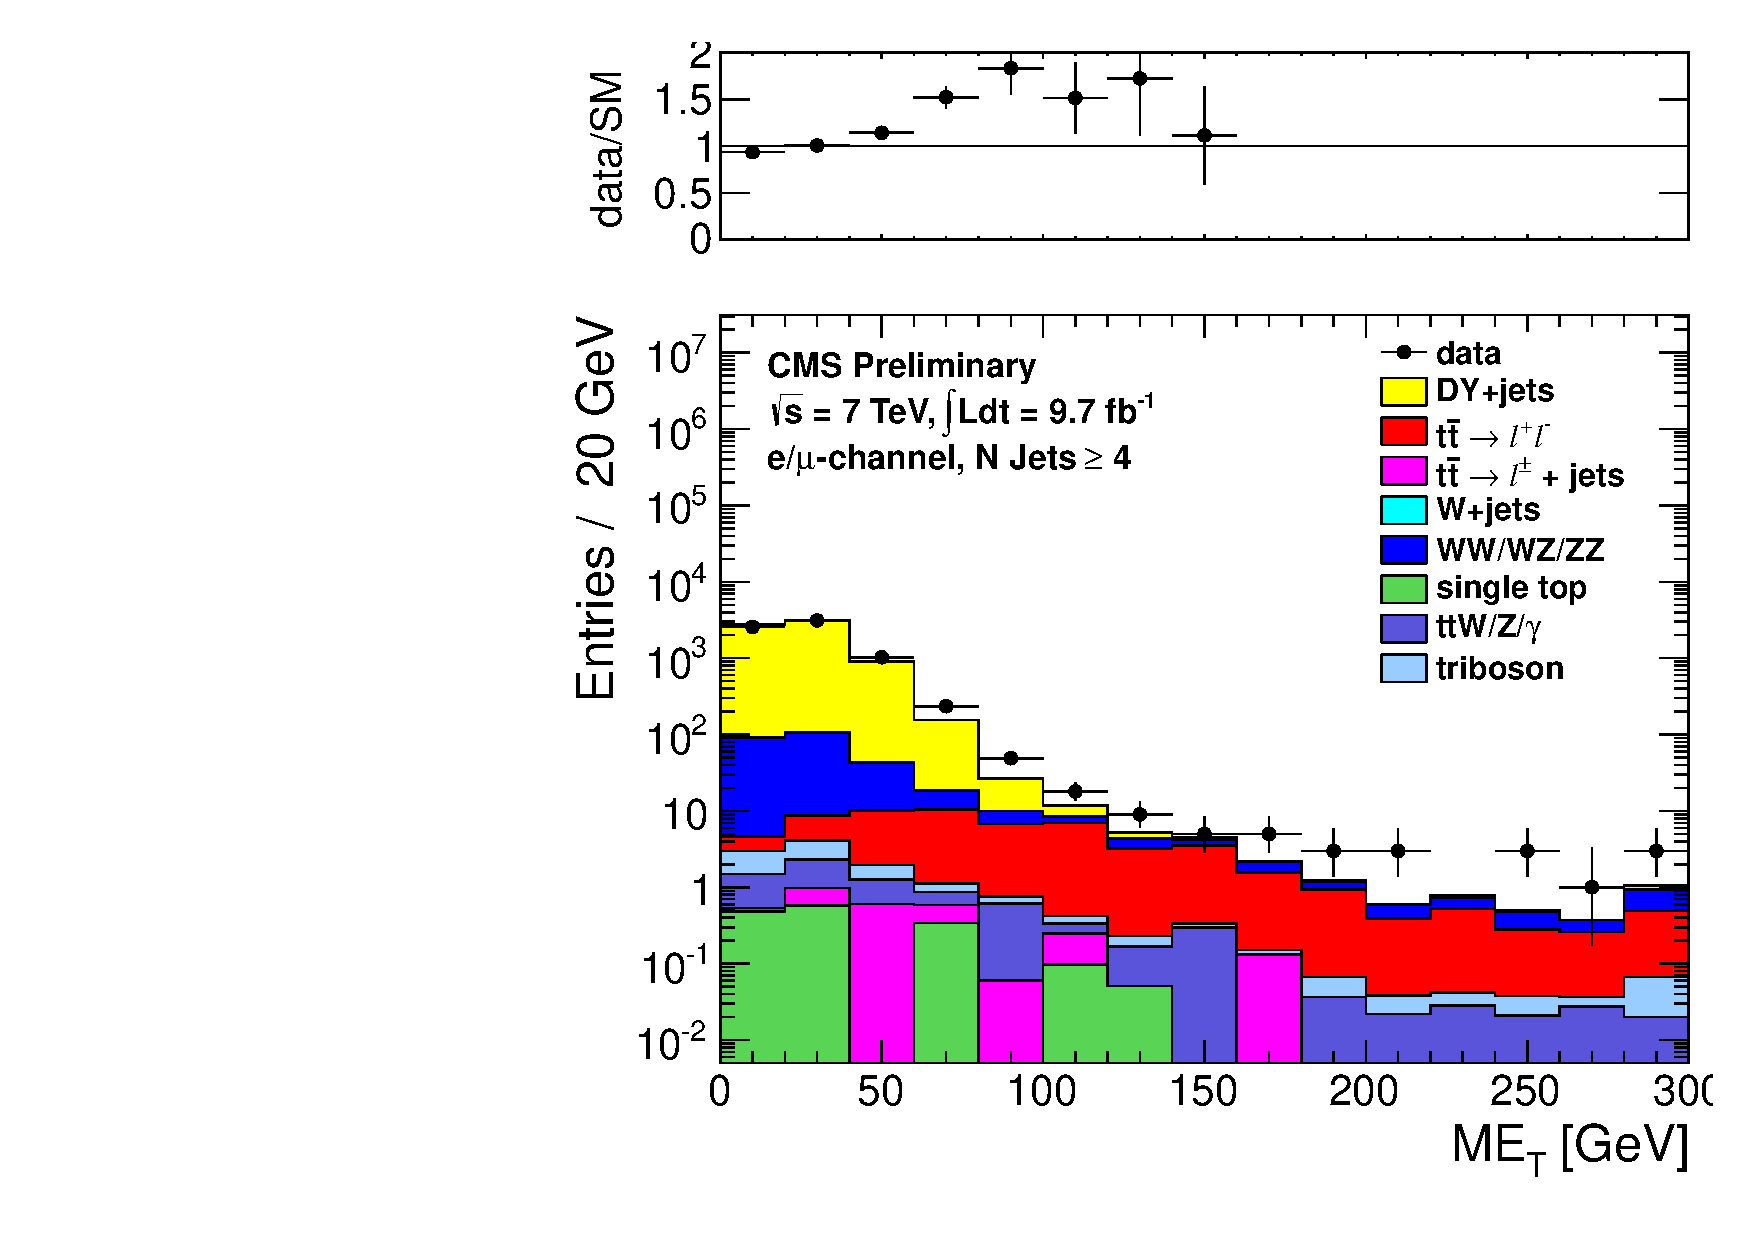
\includegraphics[width=0.5\linewidth]{plots/CR2plots/met_scaled_nj4_emucomb.pdf}%
	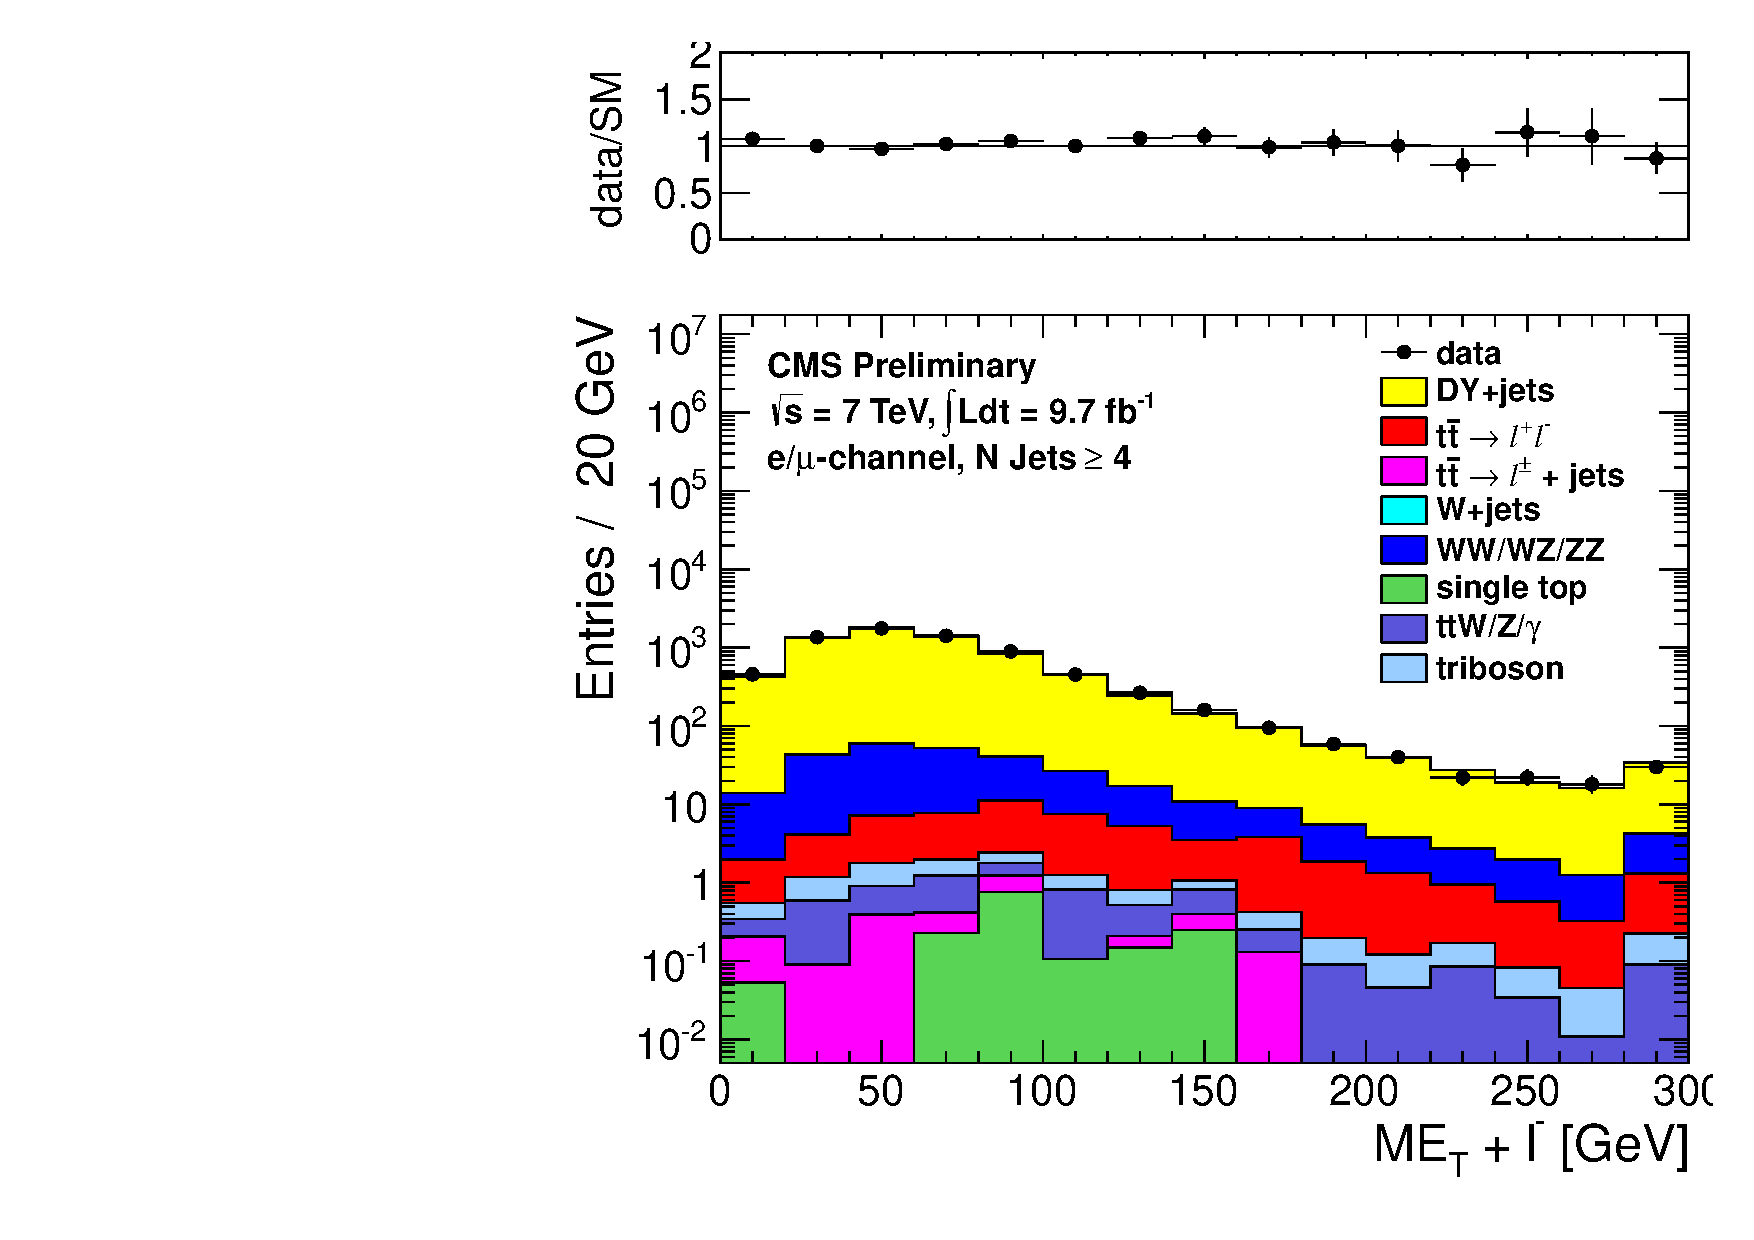
\includegraphics[width=0.5\linewidth]{plots/CR2plots/met_lepcor_scaled_nj4_emucomb.pdf}%
	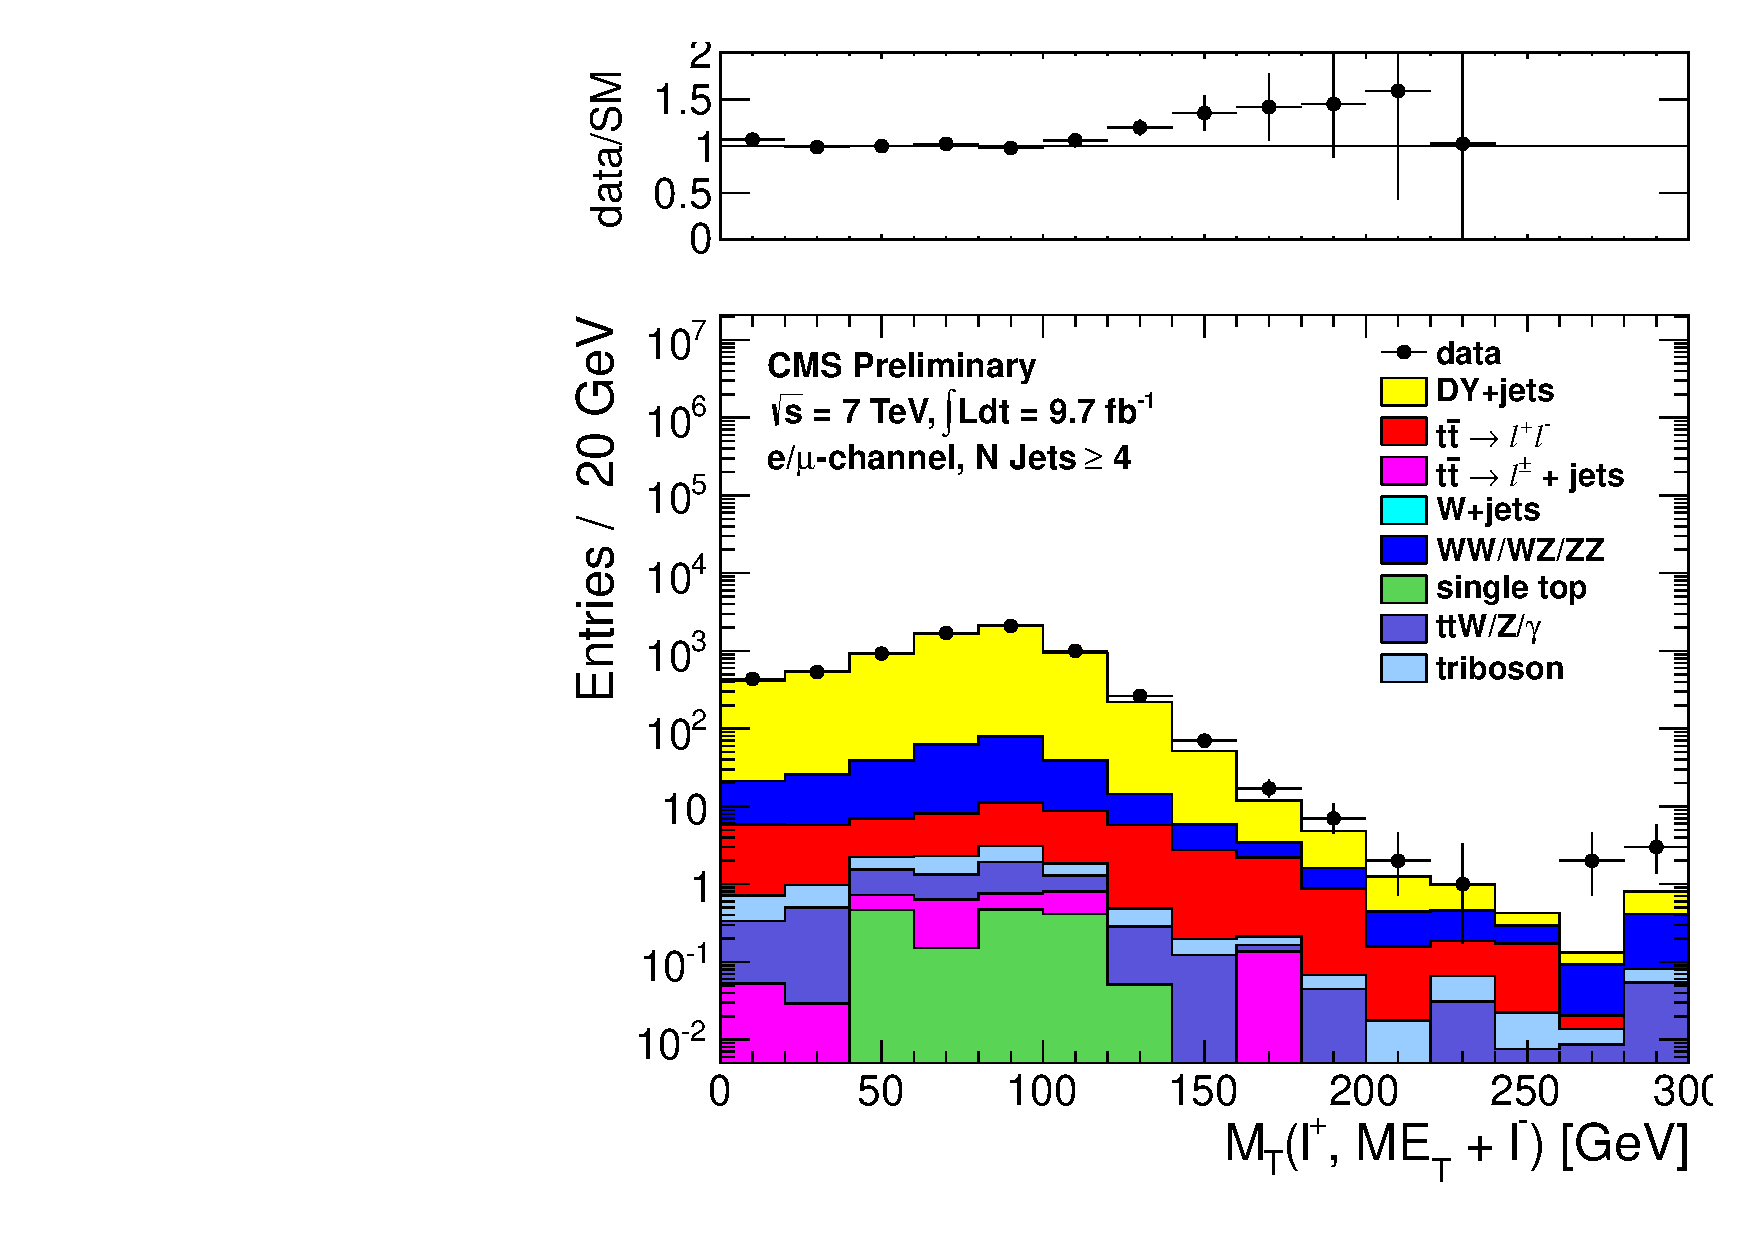
\includegraphics[width=0.5\linewidth]{plots/CR2plots/mt_lepcor_scaled_nj4_emucomb.pdf}
	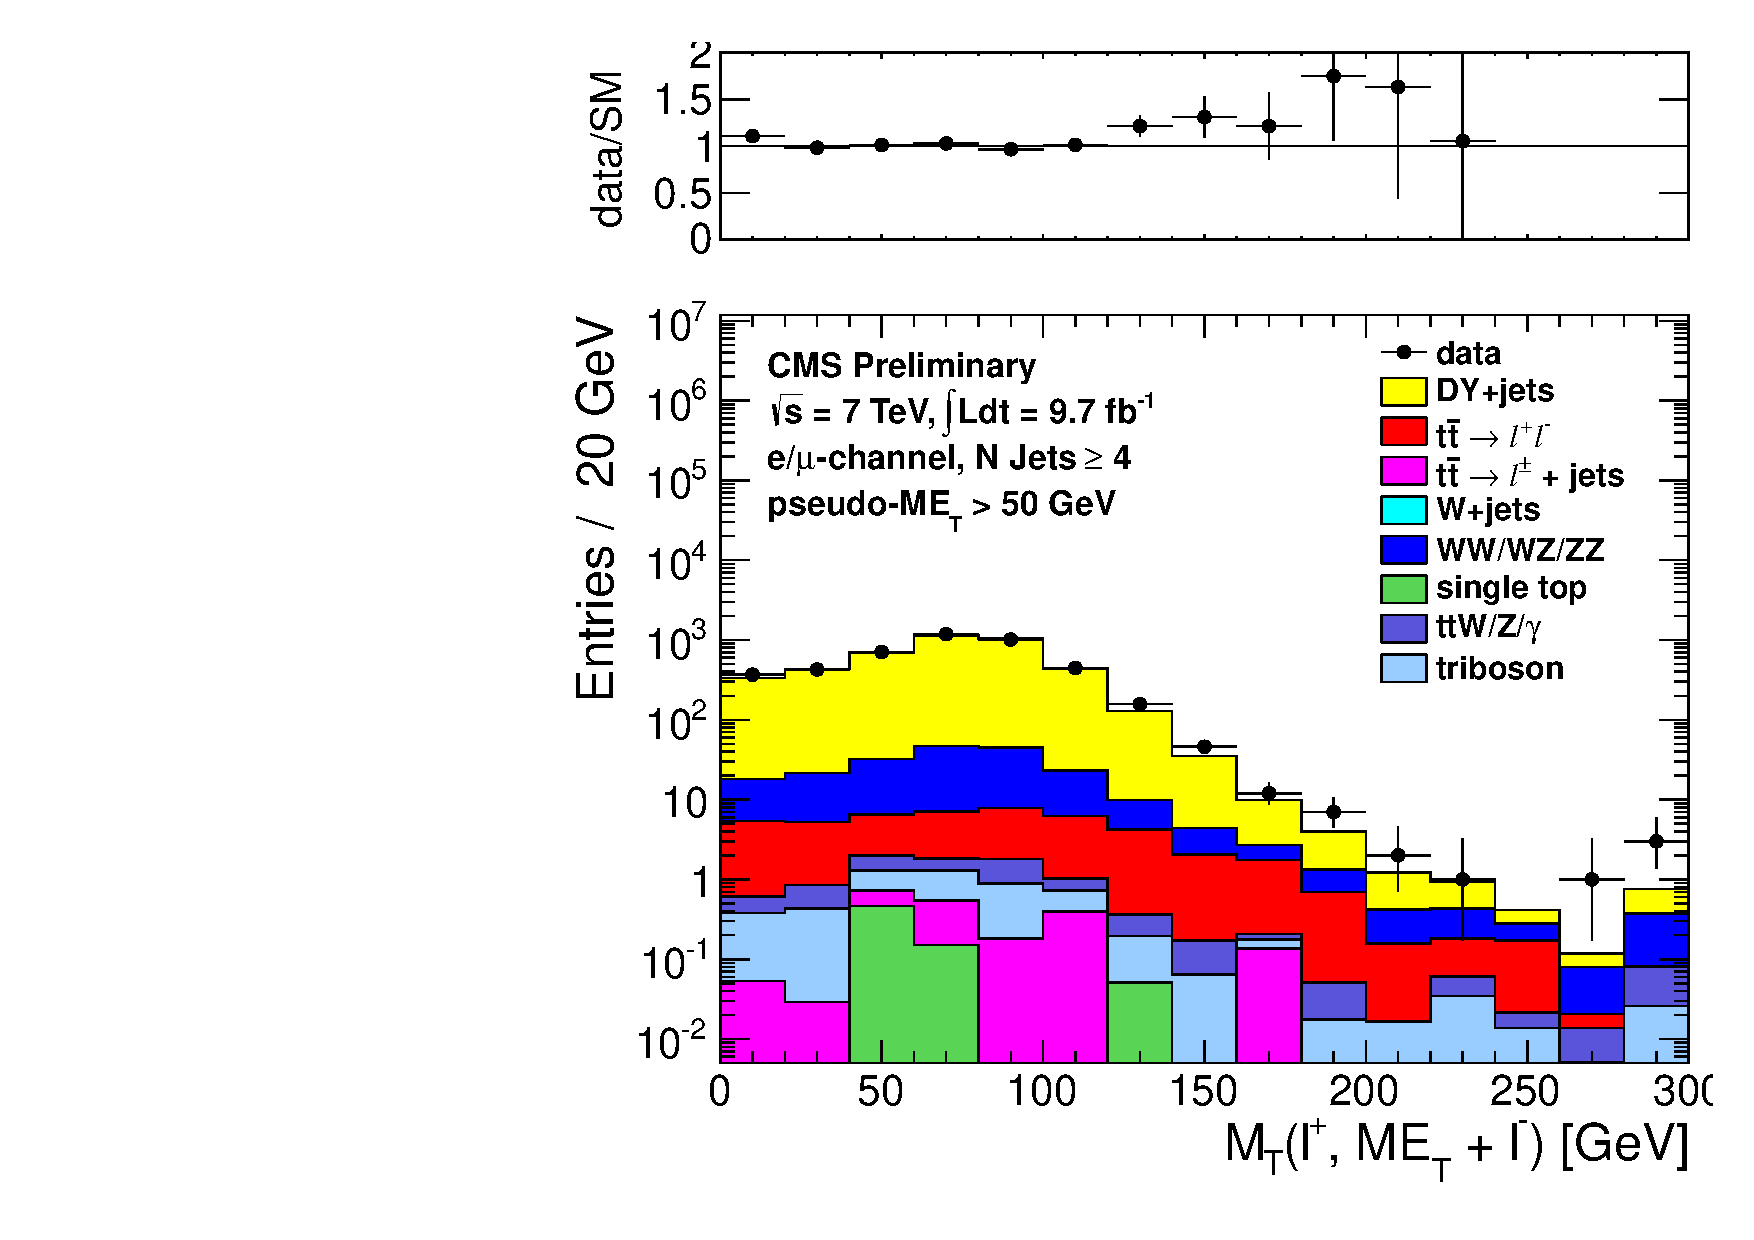
\includegraphics[width=0.5\linewidth]{plots/CR2plots/mt_lepcor_scaled_met50_nj4_emucomb.pdf}%
	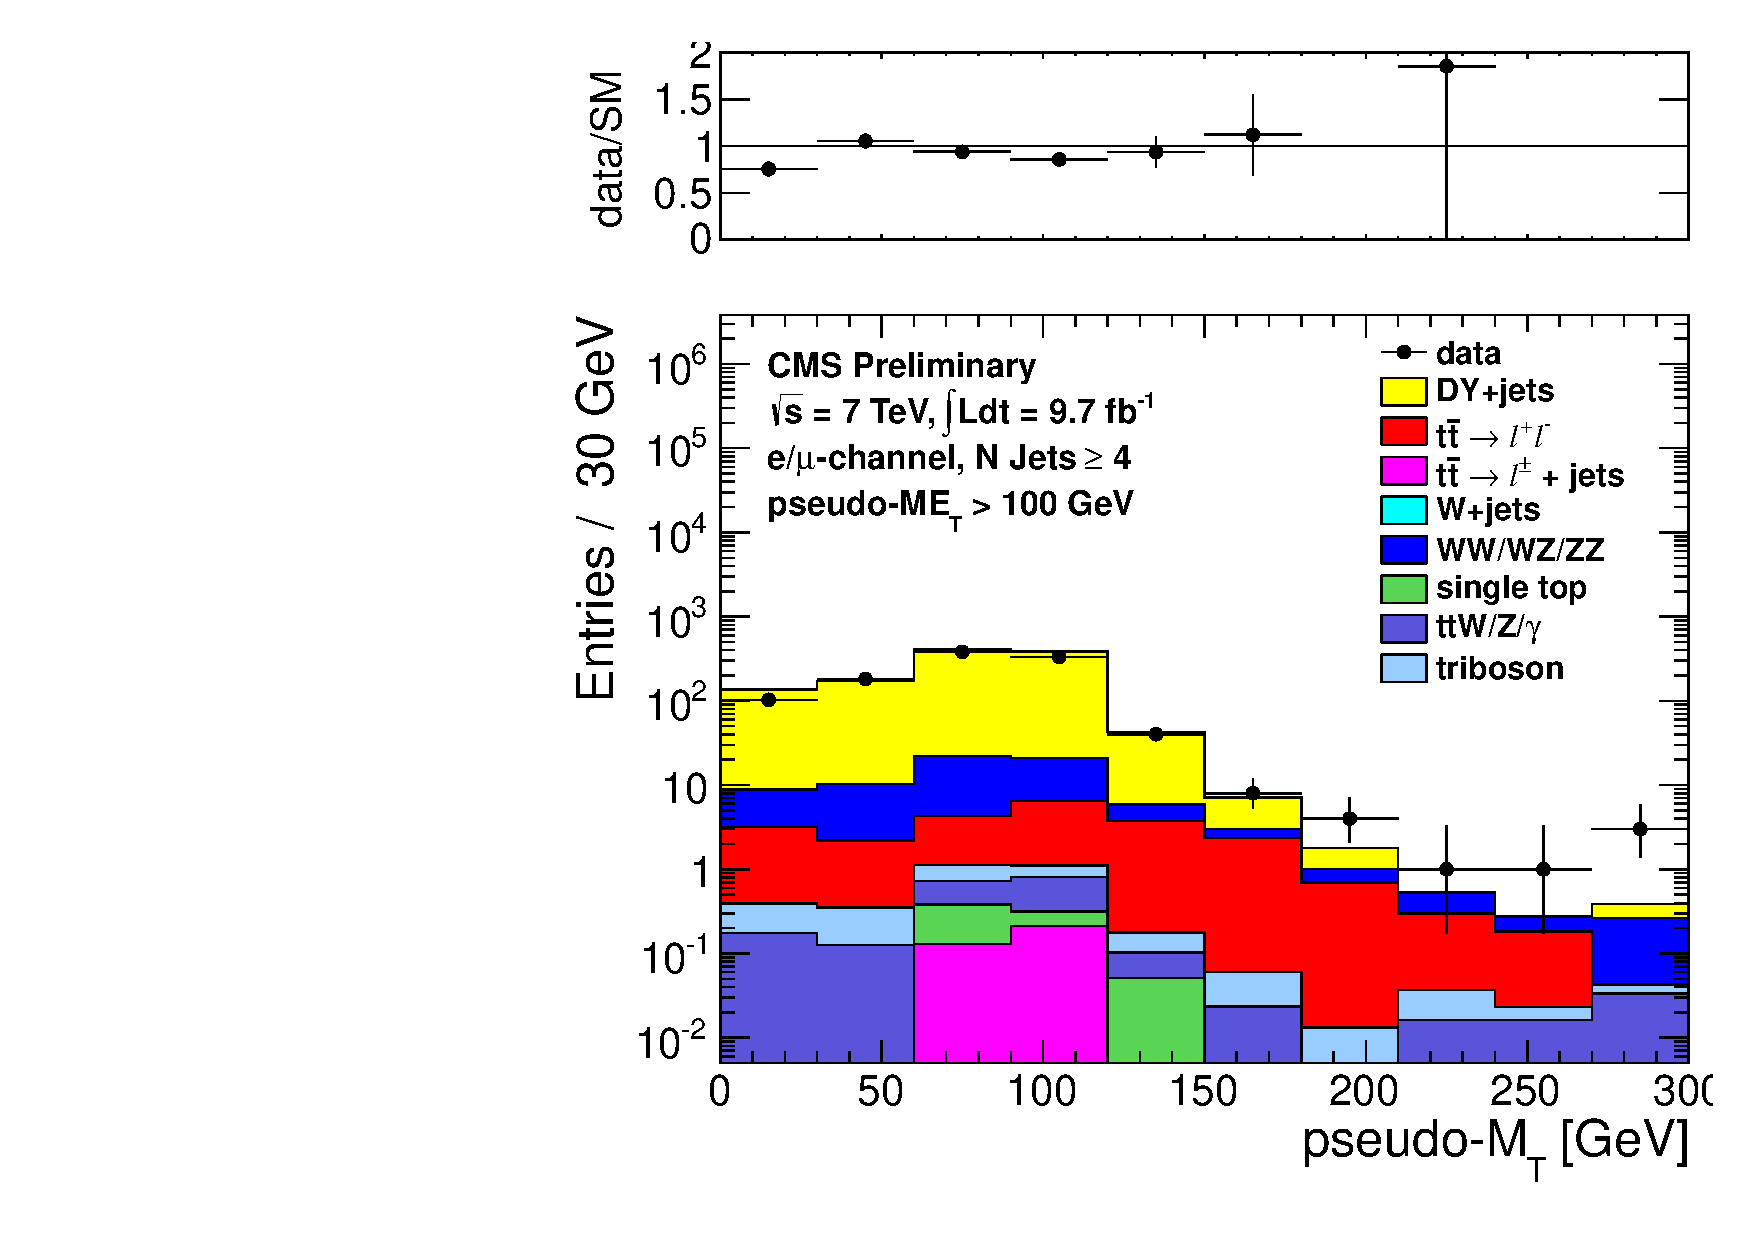
\includegraphics[width=0.5\linewidth]{plots/CR2plots/mt_lepcor_scaled_met100_nj4_emucomb.pdf}

    \caption{
      Comparison of the pseudo-\met\ (top, left), pseudo-\mt\ (top,
      right and bottom) distributions in data vs. MC for events
      satisfying the requirements of CR2, combining both the muon and
      electron channels. The pseudo-\mt\ distributions are shown
      before any additional requirements (top, right) and after
      requiring pseudo-\met $>$50 GeV (bottom, left) and pseudo-\met
      $>$ 100 GeV (bottom, right).
\label{fig:cr2met} 
}  
      \end{center}
\end{figure}

%\begin{figure}[hbt]
%  \begin{center}
%	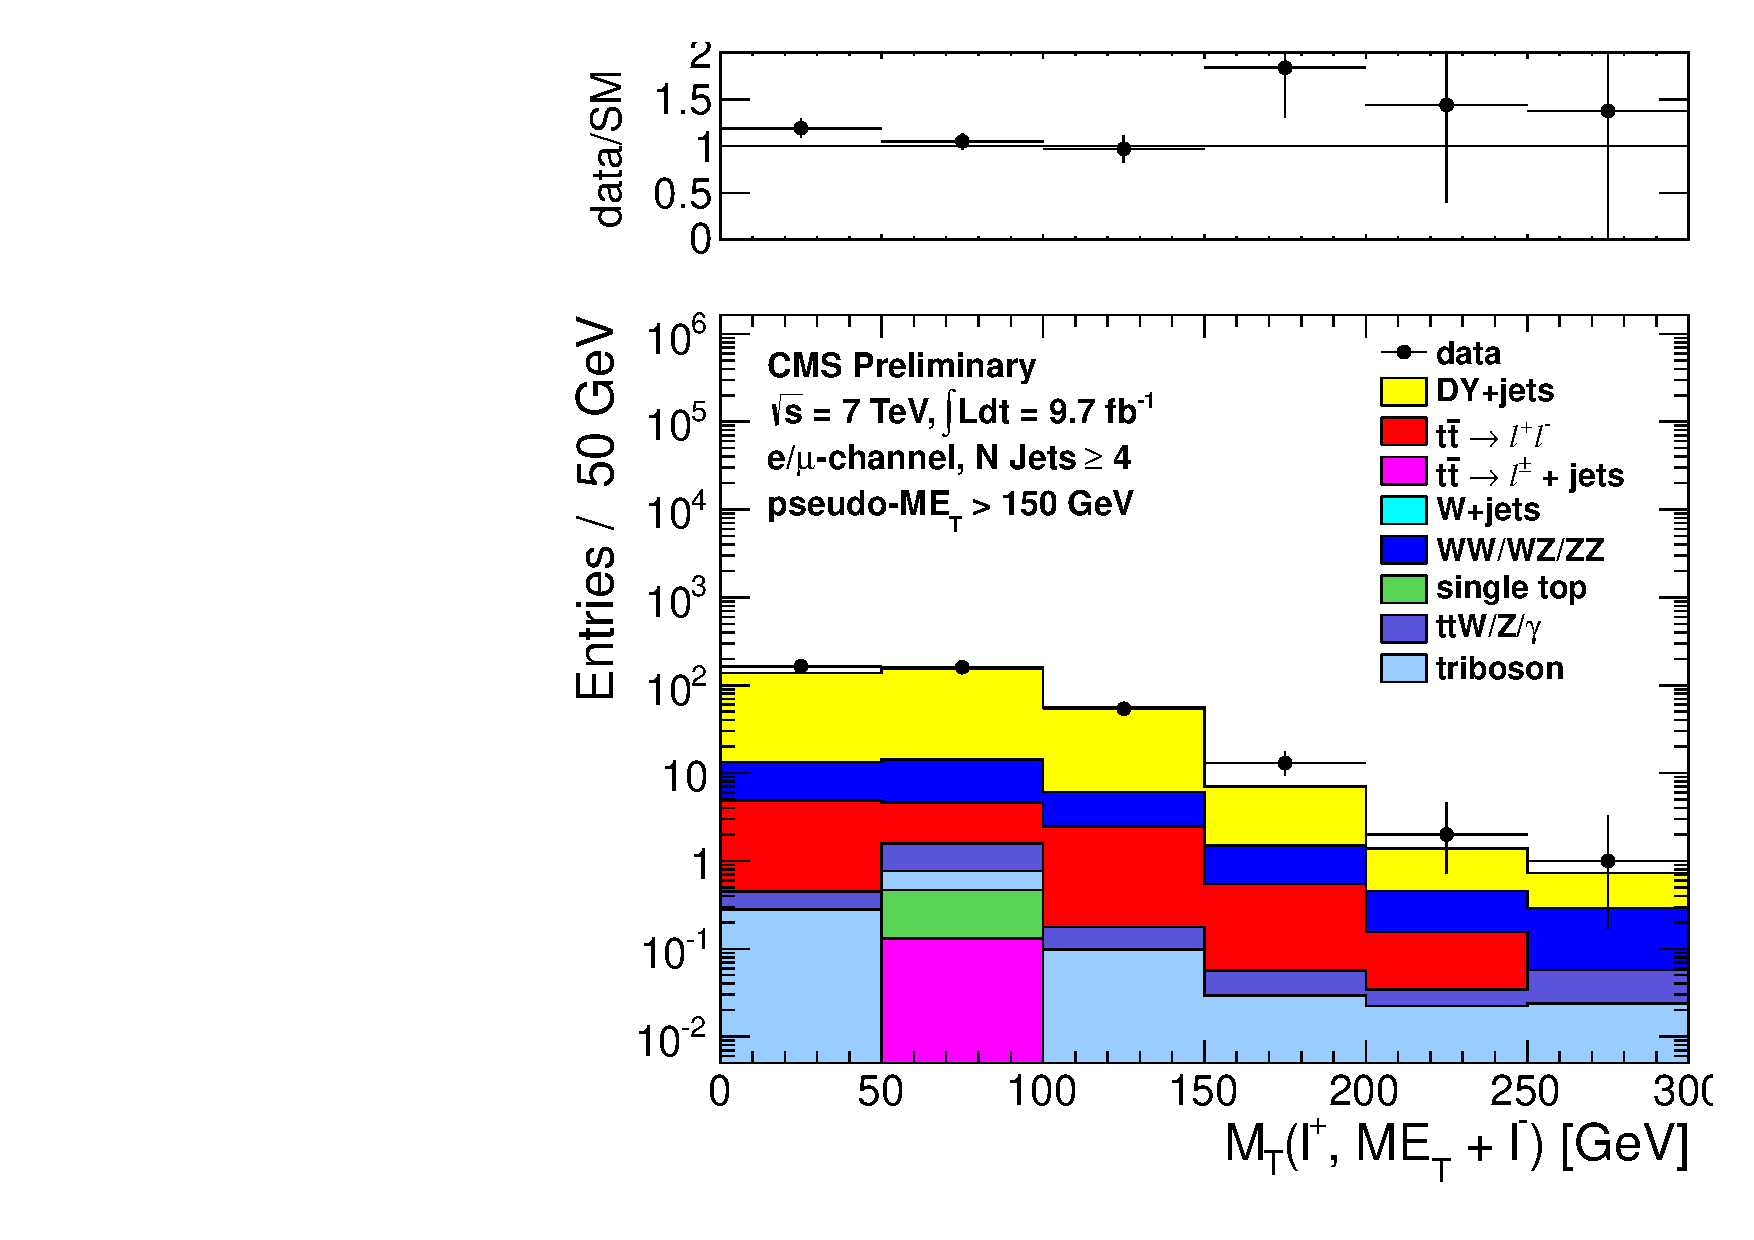
\includegraphics[width=0.5\linewidth]{plots/CR2plots/mt_lepcor_scaled_met150_nj4_emucomb.pdf}%
%	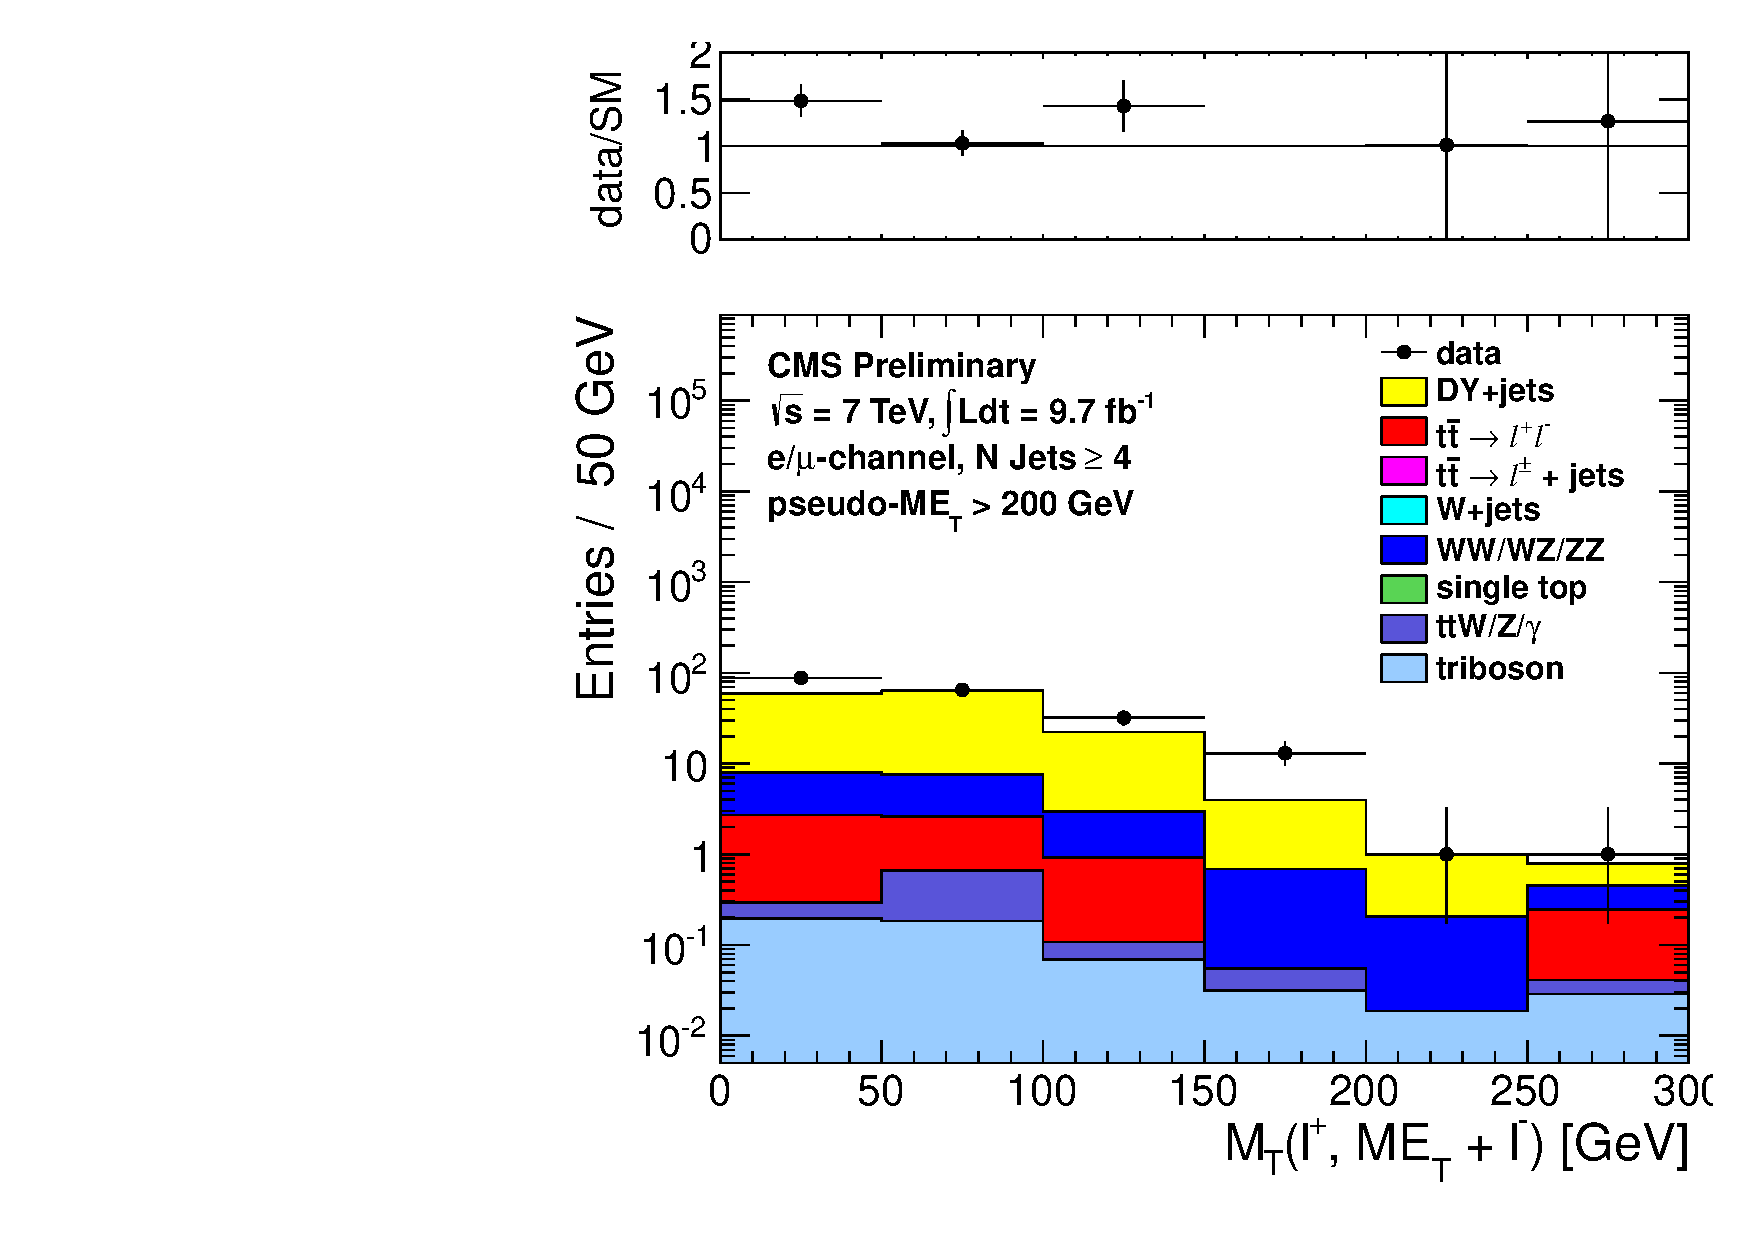
\includegraphics[width=0.5\linewidth]{plots/CR2plots/mt_lepcor_scaled_met200_nj4_emucomb.pdf}
%	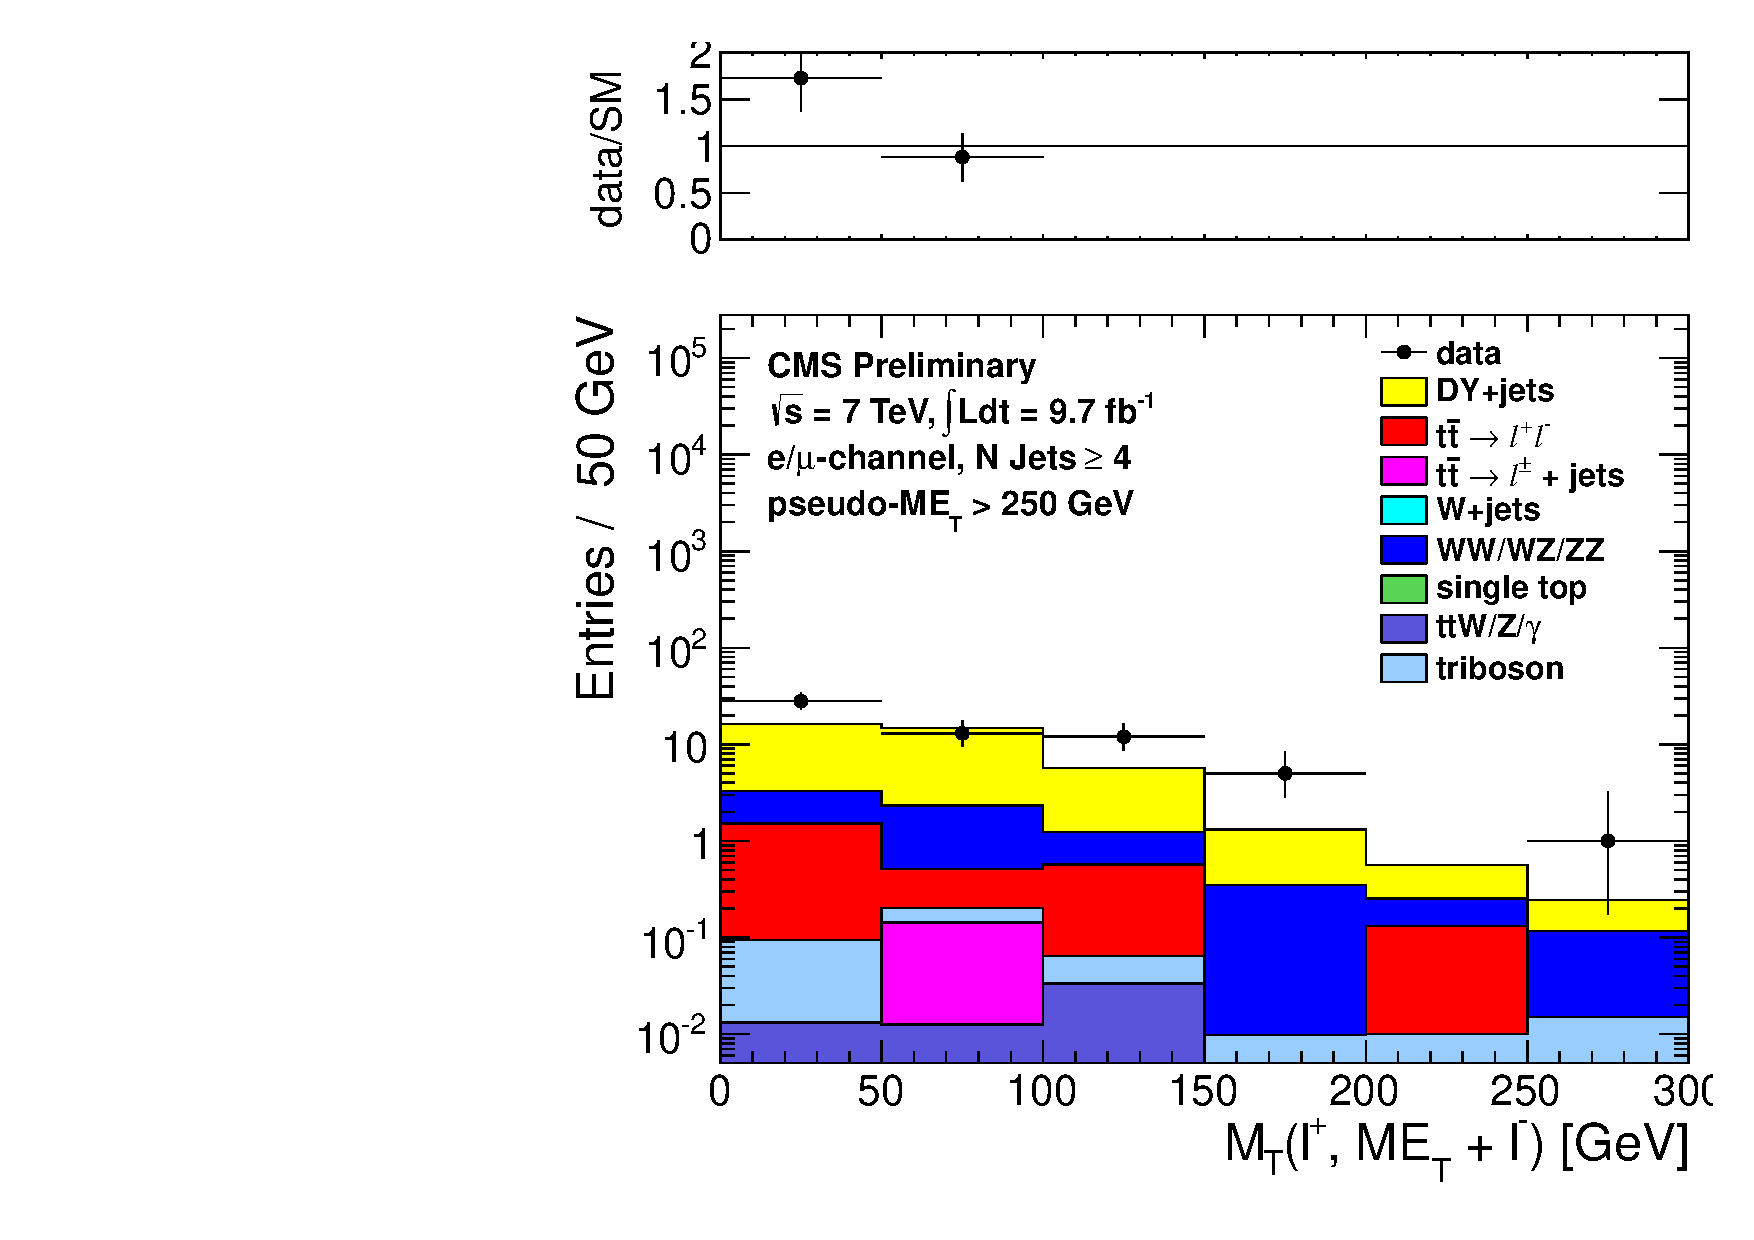
\includegraphics[width=0.5\linewidth]{plots/CR2plots/mt_lepcor_scaled_met250_nj4_emucomb.pdf}%
%	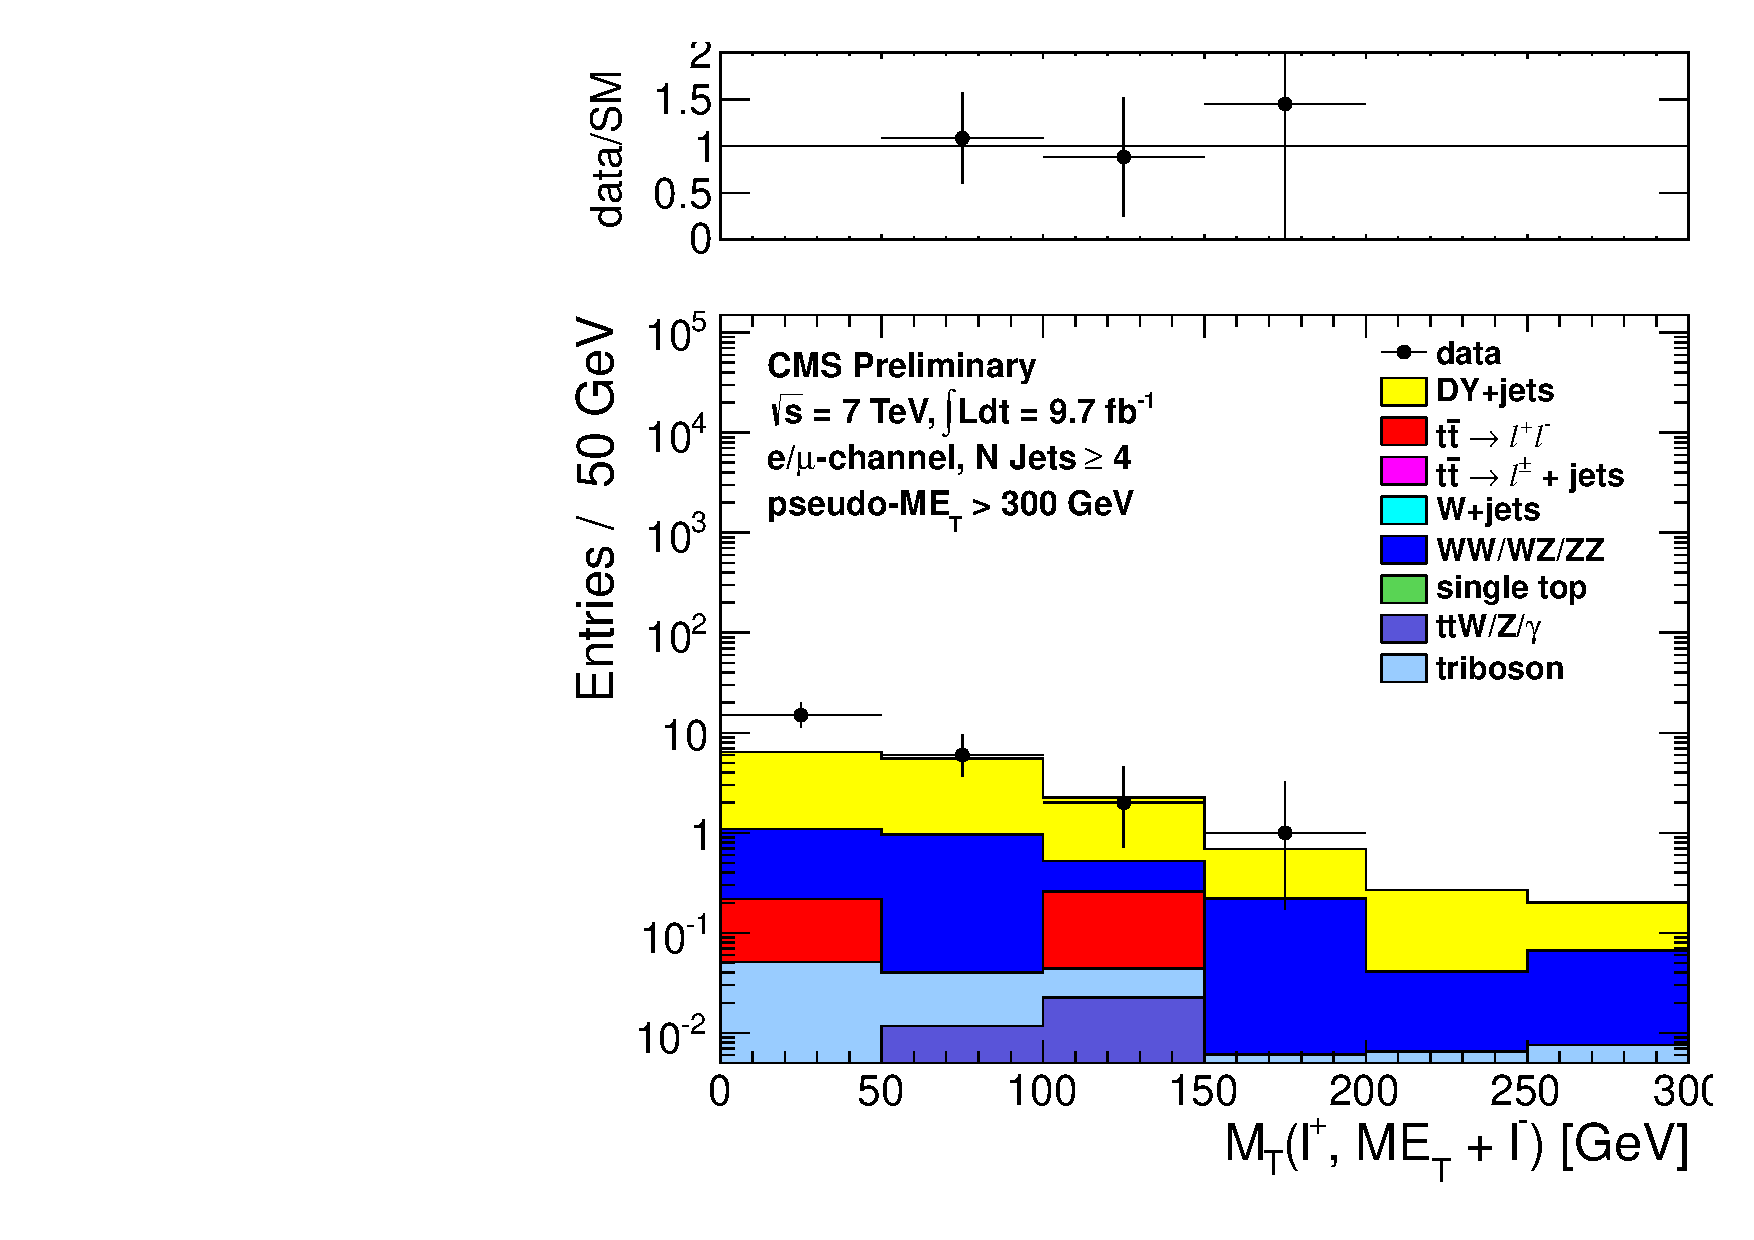
\includegraphics[width=0.5\linewidth]{plots/CR2plots/mt_lepcor_scaled_met300_nj4_emucomb.pdf}
%    \caption{
%      Comparison of the \mt\ distribution in data vs. MC for events
%      satisfying the requirements of CR2, combining both the muon and
%      electron channels. The pseudo-\met\ requirements used are
%      150 GeV (top, left), 200 GeV (top, right), 250 GeV (bottom,
%      left) and 300 GeV (bottom, right).
%\label{fig:cr2mtrest} 
%}  
%      \end{center}
%\end{figure}
\clearpage
